\documentclass{article}

% NeurIPS 2026 workshop style (double-blind)
\usepackage[dblblindworkshop]{neurips_2026}
\workshoptitle{Foundations of Language Model Security}

\usepackage[utf8]{inputenc}
\usepackage[T1]{fontenc}
\usepackage{hyperref}
\usepackage{url}
\usepackage{booktabs}
\usepackage{amsfonts}
\usepackage{amsmath}
\usepackage{amssymb}
\usepackage{amsthm}
\usepackage{nicefrac}
\usepackage{microtype}
\usepackage{xcolor}
\definecolor{safebg}{rgb}{0.85,0.93,0.85}
\definecolor{safebd}{rgb}{0.3,0.6,0.3}
\definecolor{unsafebg}{rgb}{0.95,0.85,0.85}
\definecolor{unsafebd}{rgb}{0.7,0.3,0.3}
\definecolor{pendingbg}{rgb}{0.92,0.92,0.95}
\definecolor{pendingbd}{rgb}{0.5,0.5,0.7}
\usepackage{tikz}
\usepackage{pgfplots}
\usetikzlibrary{positioning, arrows.meta, shapes.geometric, fit, calc, matrix}
\pgfplotsset{compat=1.18}

\newtheorem{definition}{Definition}
\newtheorem{theorem}{Theorem}
\newtheorem{corollary}{Corollary}

\title{Preventing Privilege Escalation in LLM Agents:\\
Provenance-Based Authority from Theory to Canonical Implementation}

\author{%
  Anonymous Author(s) \\
}

\begin{document}

\maketitle

\begin{abstract}
Large-language-model agents process information from multiple principals
while performing externally visible actions. We argue that privilege
escalation---not prompt injection per se---is the appropriate system-level
security objective. We present Influence Tracking with Extrapolated Security
(ITES), a provenance-based defence that derives effective authority from the
intersection of permissions held by all influencing principals, and the
System-Level Evaluator for Defences (SLED), which exhaustively explores
execution state spaces under worst-case model behaviour. Prior work
established the core ITES theorems and evaluated the original prototype with
SLED across approximately 1.5 million traces, observing zero privilege
escalation while preserving maximal utility. We then describe Conflux, a
canonical reimplementation with independent policy ports for read,
authorisation, visibility, and consent; argument-aware authorisation;
audience-specific disclosure; structured attribution; authenticated dynamic
planning; a serialisable formal verification subset with cone-of-influence
reduction; pinned benchmark translation; and a scoped delegation model. We
report bounded current evidence from native SLED mutation testing, formal
verification, and direction-readiness mutants, and we position the work
within the classical integrity and information-flow-control lineage.
\end{abstract}


\section{Introduction}

Large language model (LLM) agents read documents, invoke tools, and perform
externally visible actions on behalf of users. Unlike traditional software,
these agents process natural-language inputs from multiple principals,
including users, documents, databases, APIs, and other systems. Arbitrary
information may influence decisions with real-world consequences
\citep{earlycategorization}.

Prompt injection has emerged as a fundamental challenge
\citep{struq,spotlighting,neuralexec}. Model-level defences improve
instruction following but remain probabilistic: adaptive attacks may
invalidate empirical robustness
\citep{criticaleval,detectprompt,poisoningalignment,checkpointgcg}. We
instead treat \emph{privilege escalation} as the system-level security
objective: if every principal influencing an action is authorised for it,
then arbitrary model behaviour cannot increase authority
\citep{provos2003,davi2010}.

In prior work, we introduced Influence Tracking with Extrapolated Security
(ITES), a provenance-based defence that derives the effective authority of
each execution from information provenance and an existing access-control
system, and the System-Level Evaluator for Defences (SLED), which evaluates
system-level defences under worst-case model behaviour by exhaustively
exploring the reachable execution space \citep{earlycategorization}. Across
approximately 1.5 million explored traces, SLED observed no successful
privilege escalation while preserving maximal utility for all tasks
consistent with the access-control system.

This paper unifies the foundational ITES/SLED theory with the Conflux
canonical reimplementation, which extends the original prototype with
independent policy ports, argument-aware authorisation, controlled
disclosure, structured attribution, authenticated dynamic planning,
serialisable formal verification, and benchmark translation. The
contributions are:

\begin{enumerate}
  \item We argue that privilege escalation, rather than prompt injection
    itself, is the appropriate system-level security objective for LLM
    agents operating within existing access-control systems.
  \item We present ITES, whose authority-intersection rule is a
    principal-sensitive analogue of low-water-mark integrity
    \citep{biba1977,lomac}, and prove that authority is monotonically
    non-increasing as influence accumulates.
  \item We introduce SLED, which evaluates defences independently of
    language-model behaviour by exhaustively exploring the execution state
    space under worst-case assumptions.
  \item We describe the Conflux canonical architecture, which separates
    read, authorisation, visibility, and consent decisions; extends to
    argument-aware policy, audience disclosure, structured attribution,
    authenticated dynamic planning, and serialisable formal verification;
    and maintains a disabled scoped-delegation model.
  \item We report bounded current evidence from native SLED mutation
    testing, COI-reduced formal verification, and direction-readiness
    mutants, clearly distinguishing archived, bounded, and pending results.
\end{enumerate}


\section{Related Work}

\subsection{Model-Level Defences}

Model-level defences seek to make language models resist prompt injection
through improved prompting, alignment, or fine-tuning
\citep{struq,spotlighting,secalign,datasentinel}. While often effective
empirically, their security remains probabilistic and may be bypassed by
adaptive attacks \citep{criticaleval,checkpointgcg,poisoningalignment}. ITES
assumes worst-case model behaviour and derives security entirely from
system-level enforcement.

\subsection{System-Level Defences}

Several works address prompt injection through system-level enforcement.
The Dual LLM pattern separates privileged planning from untrusted parsing.
CaMeL extends this with capability tracking and developer-defined policies
enforced by a custom interpreter \citep{camel,designpatterns}. Progent
mediates tool calls with symbolic privilege control \citep{progent}. PACT
tracks argument-level provenance \citep{pact}, and FORGE enforces
history-sensitive Datalog policies \citep{forge}. ITES differs by deriving
authority directly from the organisation's existing access-control system
rather than introducing a trusted planning model, binary trust labels, or
a new policy language.

\subsection{Classical Security Lineage}

The ITES authority-intersection rule is structurally analogous to Biba's
low-water-mark contamination: consuming information from an additional
principal can preserve or reduce effective authority but cannot increase it
\citep{biba1977}. LOMAC operationalised low-water-mark integrity in
commodity systems and confronted the same utility--security tension
\citep{lomac}. Denning's lattice model provides the formal foundation: the
intersection of permission sets is a meet in the powerset lattice
\citep{denning1976}. Sabelfeld and Myers provide the vocabulary for
explicit and implicit flows \citep{sabelfeld2003}, while Myers and Liskov's
decentralized IFC moves toward multi-principal policies
\citep{myersliskov}. Declassification and endorsement mechanisms
\citep{declassification-survey,robust-declassification,attacker-control,nonmalleable-ifc}
inform Conflux's visibility and disclosure design. Conflux enriches this
lineage with authenticated principal identities and authority derived from
the organisation's current access-control state.

\subsection{Evaluation}

AgentDojo supplies realistic prompt-injection tasks and metrics
\citep{agentdojo}. Existing benchmarks evaluate robustness against known
attacks, while SLED evaluates whether a defence satisfies its intended
security objective under arbitrary model behaviour.

\begin{table}[h]
\centering
\small
\begin{tabular}{p{2.8cm}p{2.2cm}p{2.2cm}p{2.2cm}p{2.5cm}}
\toprule
& Model-level & Dual LLM & CaMeL & ITES \\
\midrule
Primary mechanism & Model robustness & Model isolation & Dual LLM + policies & Provenance + ACS \\
Security depends on model & Yes & Planning model & Planning model & No \\
Requires new policy language & No & No & Yes & No \\
Tracks & N/A & N/A & Capabilities & Principals \\
Security objective & Prevent PI & Prevent PI & Prevent PI + policies & Prevent PE \\
\bottomrule
\end{tabular}
\caption{Comparison of representative approaches. PI denotes prompt injection; PE denotes privilege escalation; ACS denotes access-control system.}
\label{tab:comparison}
\end{table}

% GENERATED FILE -- do not edit by hand.
% Source: tests/test_defence_models.py (IR model definitions)
% SHA-256: test-code
% Run: python scripts/generate_paper_figures.py

\begin{figure}[t]
\centering
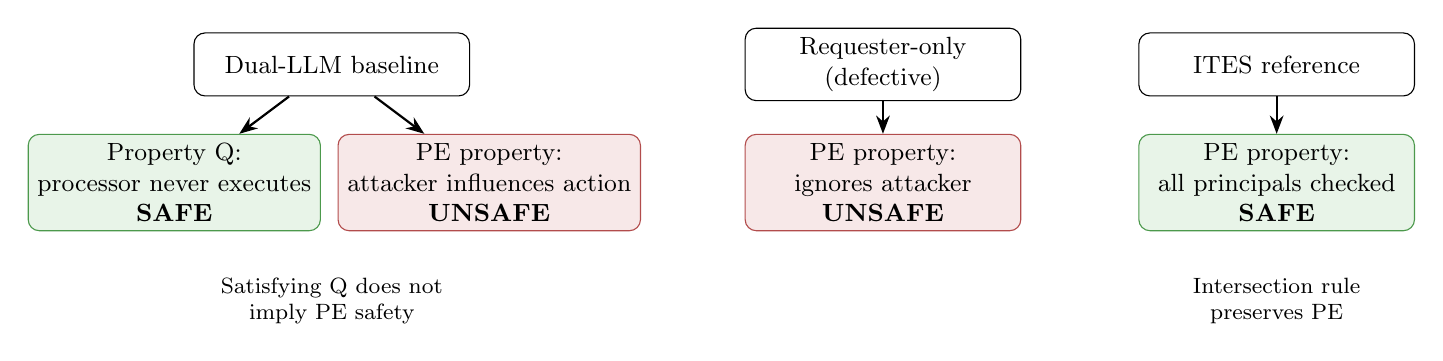
\begin{tikzpicture}[
  node distance=1.5cm and 2cm,
  state/.style={draw, circle, minimum size=1cm, font=\footnotesize},
  bad/.style={fill=unsafebg!60, draw=unsafebd},
  good/.style={fill=safebg!60, draw=safebd},
  model/.style={draw, rounded corners, minimum width=3.5cm, minimum height=0.8cm,
               font=\small, align=center},
  arrow/.style={-Stealth, thick},
]
% Colors defined globally in preamble

% --- Dual-LLM ---
\node[model] (dllm) at (0, 2) {Dual-LLM baseline};
\node[model, good] (dllm_q) at (-2, 0.5) {Property Q:\\processor never executes\\{\bf SAFE}};
\node[model, bad] (dllm_pe) at (2, 0.5) {PE property:\\attacker influences action\\{\bf UNSAFE}};

% --- Requester-only ---
\node[model] (req) at (7, 2) {Requester-only\\(defective)};
\node[model, bad] (req_pe) at (7, 0.5) {PE property:\\ignores attacker\\{\bf UNSAFE}};

% --- ITES reference ---
\node[model] (ites) at (12, 2) {ITES reference};
\node[model, good] (ites_pe) at (12, 0.5) {PE property:\\all principals checked\\{\bf SAFE}};

% Arrows
\draw[arrow] (dllm) -- (dllm_q);
\draw[arrow] (dllm) -- (dllm_pe);
\draw[arrow] (req) -- (req_pe);
\draw[arrow] (ites) -- (ites_pe);

% Annotation
\node[font=\footnotesize, align=center] at (0, -1) {Satisfying Q does not\\imply PE safety};
\node[font=\footnotesize, align=center] at (12, -1) {Intersection rule\\preserves PE};
\end{tikzpicture}
\caption{Comparative defence verification on finite IR models.  The
Dual-LLM baseline satisfies its own property Q (processor never
executes) but violates the privilege-escalation property.  The
requester-only negative control also violates PE.  The ITES reference
preserves PE.  All results are finite IR models, not
implementation-conformance evidence.}
\label{fig:defence-comparison}
\end{figure}



\section{Threat Model and Security Objective}

We consider an LLM-based agent that performs externally visible actions on
behalf of users. The agent receives information from multiple principals,
both directly through prompts and indirectly through documents, APIs, and
tool outputs. Any principal may provide arbitrary inputs; we make no
assumptions about the model's ability to distinguish instructions from data
or resist prompt injection. The enforcement mechanism and access-control
system (ACS) are assumed correct and uncompromised.

\subsection{Access-Control System}

We model the ACS as the tuple $(A, U, D, P, W, R)$, where $A$ is the set of
parameterised actions, $U$ is the set of principals, $D$ is the set of data
objects, $P \subseteq U \times A$ is the permission relation, $W
\subseteq D \times U$ specifies authorship, and $R \subseteq D \times U$
specifies read access \citep{abac}. For principal $u$ and action $a$,
$P(u, a)$ holds iff $u$ is authorised to perform $a$.

\subsection{Security Objective}

\begin{definition}[Influencing Principal]
A principal $u$ influences an action if information originating from $u$
contributes, directly or indirectly, to the execution that produces the
action.
\end{definition}

\begin{definition}[Privilege Escalation]
Privilege escalation occurs iff the agent performs an action $a \in A$ for
which there exists an influencing principal $u \in U$ such that $\neg
P(u, a)$.
\end{definition}

Under this formulation, security depends only on provenance and the current
access-control state, not on the source or mechanism of influence. Prompt
injection is one possible source of influence; ITES treats it uniformly with
any other.


\section{ITES: Provenance-Based Authority}

The central principle of ITES is that every execution inherits the
effective authority implied by the provenance of its inputs. For an
execution $e$ whose direct inputs are data objects $ds \subseteq D$, the
\emph{Principal Context} (influence set in prior work) is:
\[
\mathrm{PC}(e) = \bigcup_{d \in ds} \{u \in U \mid W(d, u)\}.
\]
Objects produced by an execution inherit its complete Principal Context.
Influence accumulates monotonically: once a principal influences a
computation, that influence persists unless a trusted provenance mechanism
removes it. Under the conservative model, influence is never removed.

\subsection{Authorisation Rule}

Given an execution $e$ with Principal Context $\mathrm{PC}(e)$, ITES permits
an action $a \in A$ iff:
\[
\forall u \in \mathrm{PC}(e),\; P(u, a).
\]
Equivalently, the effective authority is the intersection of the permission
sets of all influencing principals. The Conflux extension adds a
non-empty-context condition: an action is blocked if $\mathrm{PC}(e) =
\varnothing$, preventing vacuous authority.

\subsection{Maximal Secure Authorisation}

\begin{theorem}[Maximal Secure Authorisation]
ITES authorises the maximal set of actions that can be permitted without
allowing privilege escalation.
\end{theorem}

\begin{proof}[Proof sketch]
ITES authorises exactly $\bigcap_{u \in \mathrm{PC}(e)} \{a \mid P(u, a)\}$.
Any strict superset must include an action $a$ for which some influencing
principal $u$ lacks permission, satisfying Definition~2.
\end{proof}

\subsection{Authority Monotonicity}

\begin{theorem}[Authority Monotonicity]
If $\mathrm{PC}(e_1) \subseteq \mathrm{PC}(e_2)$, then
$\mathrm{Permitted}(\mathrm{PC}(e_2)) \subseteq
\mathrm{Permitted}(\mathrm{PC}(e_1))$.
\end{theorem}

\begin{proof}[Proof sketch]
Adding influencing principals introduces additional constraints; the
intersection can only shrink or remain unchanged.
\end{proof}

\begin{corollary}[Security Guarantee]
Under the threat model of Section~3, and assuming correct enforcement of
influence tracking, provenance, and access-control checks, ITES prevents
privilege escalation.
\end{corollary}

The guarantee is independent of the source of influence. Prompt injection,
retrieved documents, compromised tools, and arbitrary model behaviour are
treated uniformly: once information contributes to an execution, the
authority of that execution is constrained by the permissions of the
corresponding principals.


\section{SLED: Worst-Case Evaluation}

Existing prompt-injection benchmarks measure robustness against a finite
collection of attacks. SLED instead evaluates whether a system-level
defence correctly enforces its security properties under arbitrary model
behaviour.

\subsection{State-Space Exploration}

SLED treats each execution as a nondeterministic black box that may produce
any behaviour consistent with the system interface. A system state contains
the environment, the ACS, available data, accumulated influence, pending
executions, and possible actions. Beginning from an initial state, SLED
enumerates every action that may result from each pending execution,
updates the environment, propagates influence, and schedules further
executions. Exploration continues until every reachable state is visited
or a bound is reached.

% GENERATED FILE -- do not edit by hand.
% Source: output\runs\sled-canon-env01\verification.json; output\runs\smoke\result.json
% SHA-256: 0fdaa54c2c7d0a532383372efaab93ef885d4e589d5f46b60415f6330709f18e;9490ec77231e64c8ae30164244dd3b1def207fc55027b4eff7f1d9cc1713ae44
% Run: python scripts/generate_paper_figures.py

\begin{figure}[t]
\centering
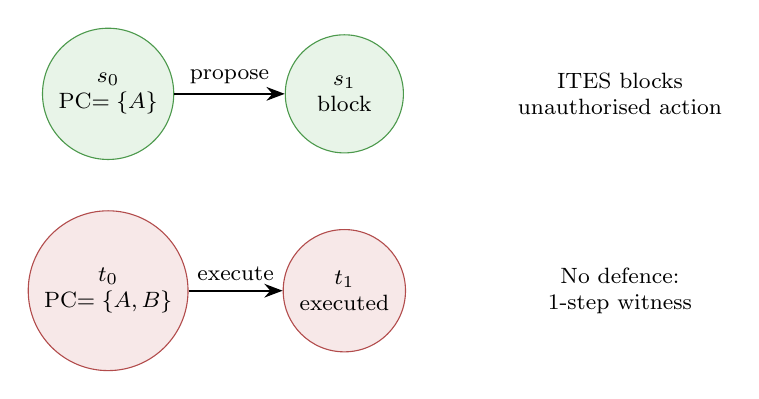
\begin{tikzpicture}[
  node distance=2.5cm,
  state/.style={draw, circle, minimum size=1.5cm, font=\footnotesize, align=center},
  good/.style={fill=safebg!60, draw=safebd},
  bad/.style={fill=unsafebg!60, draw=unsafebd},
  arrow/.style={-Stealth, thick},
  label/.style={font=\footnotesize, align=center, midway, above},
]
% Colors defined globally in preamble

% ITES path (safe)
\node[state, good] (s0) at (0, 0) {$s_0$\\PC$=\{A\}$};
\node[state, good] (s1) at (3, 0) {$s_1$\\block};
\draw[arrow] (s0) -- node[label] {propose} (s1);

% No-defence path (unsafe, counterexample)
\node[state, bad] (t0) at (0, -2.5) {$t_0$\\PC$=\{A,B\}$};
\node[state, bad] (t1) at (3, -2.5) {$t_1$\\executed};
\draw[arrow] (t0) -- node[label] {execute} (t1);

% Annotation
\node[font=\footnotesize, align=center] at (6.5, 0) {ITES blocks\\unauthorised action};
\node[font=\footnotesize, align=center] at (6.5, -2.5) {No defence:\\1-step witness};
\end{tikzpicture}
\caption{SLED state-space exploration on the canonical
confidential-handoff environment (2 states, 1 transition, safe at
depth~12).  Top: ITES blocks the unauthorised
action (SAFE).  Bottom: without defence, a one-step counterexample
reaches execution (UNSAFE).  Smoke result: 2 proposed, 1 authorised, 1 blocked.}
\label{fig:sled-state-space}
\end{figure}


\subsection{Archived Prototype Results}

In prior work, SLED evaluated the original ITES prototype across three
representative environments, exploring approximately 1.5 million execution
traces. No successful privilege escalation or information exfiltration was
observed, while maximal utility was preserved for all tasks authorised by
the ACS. These results apply to the prior prototype and not to the
refactored canonical kernel; current evidence is reported in Section~8.

\subsection{Native SLED in Conflux}

The Conflux reimplementation provides native SLED with breadth-first
exploration, canonical state keys, deduplication, retained bounds, and
shortest counterexamples. Verdicts are \texttt{SAFE} (exhausted finite
model), \texttt{BOUNDED\_SAFE} (truncated), \texttt{UNSAFE}
(counterexample found), or \texttt{UNKNOWN} (modelling failure).

% GENERATED FILE -- do not edit by hand.
% Source: output\runs\native-sled-reproduction-v1\result.json
% SHA-256: f760a47ec6ae2418d60dd0d19425d07a0101547b1e63f94c53bea12c288739ba
% Run: python scripts/generate_paper_figures.py

\begin{figure}[t]
\centering
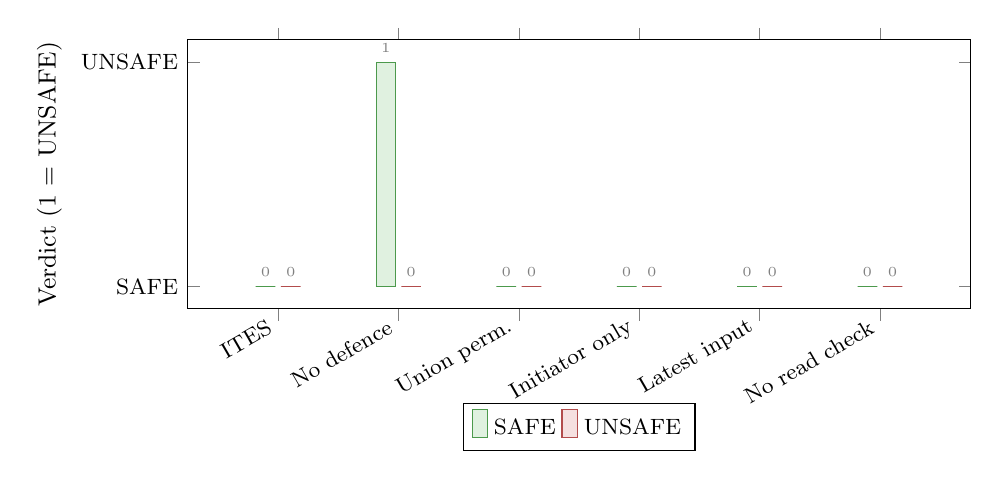
\begin{tikzpicture}
\begin{axis}[
    width=0.95\columnwidth,
    height=5cm,
    ybar,
    bar width=0.25cm,
    enlarge x limits=0.15,
    ylabel={Verdict (1 = UNSAFE)},
    ylabel style={font=\small},
    xlabel={Defence variant},
    xlabel style={font=\small},
    symbolic x coords={ITES,No defence,Union perm.,Initiator only,Latest input,No read check},
    xtick=data,
    x tick label style={font=\footnotesize, rotate=30, anchor=east},
    ytick={0,1},
    yticklabels={SAFE, UNSAFE},
    yticklabel style={font=\footnotesize},
    nodes near coords,
    nodes near coords style={font=\tiny, color=gray},
    legend style={at={(0.5,-0.35)}, anchor=north, legend columns=3, font=\footnotesize},
    legend image code/.code={
      \draw[#1] (0cm,-0.1cm) rectangle (0.2cm,0.25cm);
    },
]
\addplot[fill=safebg!80, draw=safebd] coordinates {
    (ITES,0) (No defence,1) (Union perm.,0) (Initiator only,0) (Latest input,0) (No read check,0)
};
\addplot[fill=unsafebg!80, draw=unsafebd] coordinates {
    (ITES,0) (No defence,0) (Union perm.,0) (Initiator only,0) (Latest input,0) (No read check,0)
};
\legend{SAFE, UNSAFE}
\end{axis}
\end{tikzpicture}
\caption{Native SLED verdicts on the canonical confidential-handoff
fixture.  Only \emph{no defence} produces an UNSAFE verdict with a
one-step counterexample; ITES and all corrected variants are SAFE.
Five of five defective monitors are detected across three fixture
pairs (60 transitions total).}
\label{fig:native-sled}
\end{figure}
% Canonical data: 3 pairs, 6 defences
% Negative controls killed: 5/5



\section{Conflux: Canonical Architecture and Extensions}

Conflux refactors the original prototype into a canonical security kernel
with one dependency direction and one mediation boundary. Immutable domain
values represent principals, Principal Contexts, permissions, resources,
artefacts, provenance, sessions, and actions. The ITES kernel is pure:
model proposals cannot assert or narrow their Principal Context,
alternative branches share an immutable parent, and effect execution
requires an exact decision certificate.

\subsection{Independent Policy Ports}

Authorisation, read access, visibility, and consent are separate decisions.
Consent cannot override authority; visibility cannot override read policy.
This separation prevents a single policy dimension from manufacturing
authority for another.

\subsection{Argument-Aware Authorisation}

Trusted action-argument roles carry provenance independently of the
proposing execution. Pointwise selector policy checks each principal for
each argument component, preventing authority borrowing through content or
consent.

\subsection{Audience-Specific Disclosure and Attribution}

Deterministic redaction produces audience-specific event views that do not
copy hidden payload fields. Structured attribution records are
evidence-derived rather than model-asserted: trusted model explanations are
rejected in favour of provenance, context, and policy records.

\subsection{Authenticated Dynamic Planning}

Open-ended plans use authenticated operation catalogues, typed bindings,
immutable graph patches, explicit bounded loops, and continuations. Every
grounded effect is re-mediated by ITES at action time; the planner cannot
manufacture authority. Generated code is inert data submitted to a mediated
sandbox capability, not trusted control flow. Security is a hard selection
constraint; eligible plans are then ordered by utility, authority
footprint, sensitive observations, and cost.

\subsection{Scoped Delegation}

The delegation model supports exact issuer, beneficiary, operation,
resource, and argument bindings with expiry, revocation, and atomic
one-use consumption. Delegation remains \emph{runtime-disabled}: ITES still
denies delegation operations. The model exists for bounded verification
only.

\subsection{Serialisable Formal Verification}

A serialisable verification IR supports a reference interpreter, runtime
differential tests, optional Z3 bounded model checking, and a nuXmv
Boolean subset. Property-scoped cone-of-influence (COI) reduction closes
transitively over guards and dependencies. Reduction claims require matching
reference verdicts and a liftable unsafe witness.

% GENERATED FILE -- do not edit by hand.
% Source: output\runs\sled-coi-reduction-v1\result.json
% SHA-256: 8f5ab582212da4ad95e08c3ce0c32b9ce1e36fce808df813ada6008b6ae9e1ca
% Run: python scripts/generate_paper_figures.py

\begin{figure}[t]
\centering
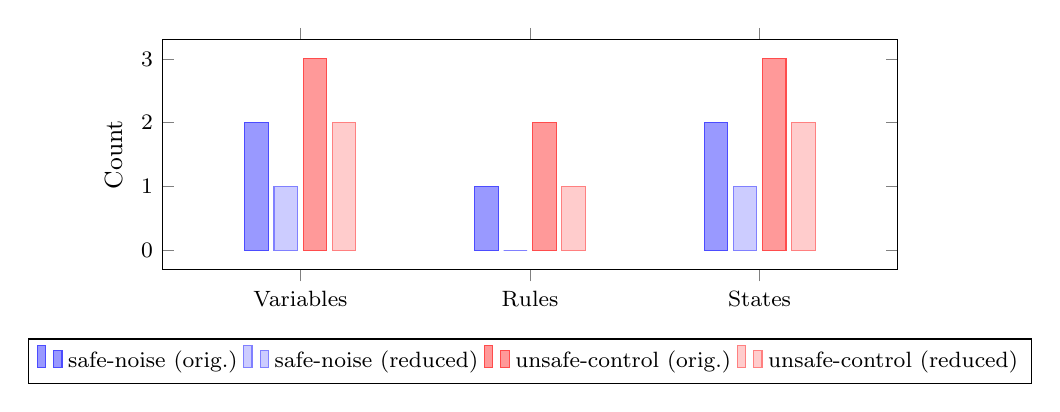
\begin{tikzpicture}
\begin{axis}[
    width=0.9\columnwidth,
    height=4.5cm,
    ybar,
    bar width=0.3cm,
    enlarge x limits=0.3,
    ylabel={Count},
    ylabel style={font=\small},
    symbolic x coords={Variables, Rules, States},
    xtick=data,
    x tick label style={font=\footnotesize},
    yticklabel style={font=\footnotesize},
    legend style={at={(0.5,-0.3)}, anchor=north, legend columns=4, font=\footnotesize},
]
\addplot[fill=blue!40, draw=blue!70] coordinates {
    (Variables, 2) (Rules, 1) (States, 2)
};
\addplot[fill=blue!20, draw=blue!50] coordinates {
    (Variables, 1) (Rules, 0) (States, 1)
};
\addplot[fill=red!40, draw=red!70] coordinates {
    (Variables, 3) (Rules, 2) (States, 3)
};
\addplot[fill=red!20, draw=red!50] coordinates {
    (Variables, 2) (Rules, 1) (States, 2)
};
\legend{safe-noise (orig.), safe-noise (reduced), unsafe-control (orig.), unsafe-control (reduced)}
\end{axis}
\end{tikzpicture}

\vspace{2mm}
\small
\begin{tabular}{lccccc}
\toprule
Fixture & Variables & Rules & States & Verdict (orig/red) & Agree \\
\midrule
safe-noise & 2 $\to$ 1 & 1 $\to$ 0 & 2 $\to$ 1 & safe / safe & True \\
unsafe-control & 3 $\to$ 2 & 2 $\to$ 1 & 3 $\to$ 2 & unsafe / unsafe & True \\
\bottomrule
\end{tabular}
\caption{Cone-of-influence reduction on two finite IR fixtures.
Reduction removes the noise variable and its associated rules in both
cases; verdicts agree between original and reduced models.  The unsafe
witness lifts to the original model.}
\label{fig:coi-reduction}
\end{figure}


% GENERATED FILE -- do not edit by hand.
% Source: output\runs\verify-coi-safe\formal-verification-original.json (sha: cc02ebdacc4b); output\runs\verify-coi-unsafe\formal-verification-original.json (sha: b69638ddd900); output\runs\verify-coi-original-safe\formal-verification-original.json (sha: e409c5461ace); output\runs\verify-coi-original-unsafe\formal-verification-original.json (sha: d45a08a5dbfc)
% SHA-256: multiple
% Run: python scripts/generate_paper_figures.py

\begin{figure}[t]
\centering
\small
\begin{tabular}{lccc}
\toprule
Fixture & Bound & CX steps & Verdict \\
\midrule
safe (basic) & 3 & 0 & \textcolor{green!60!black}{SAFE} \\
unsafe (basic) & 3 & 2 & \textcolor{green!60!black}{SAFE} \\
safe-noise (COI) & 4 & 0 & \textcolor{green!60!black}{SAFE} \\
unsafe-control (COI) & 4 & 2 & \textcolor{green!60!black}{SAFE} \\
\bottomrule
\end{tabular}

\vspace{2mm}
\begin{tabular}{lcc}
\toprule
COI fixture & States (orig $\to$ reduced) & Z3 agrees \\
\midrule
safe-noise & 2 $\to$ 1 & True \\
unsafe-control & 3 $\to$ 2 & True \\
\bottomrule
\end{tabular}
\caption{Z3 bounded model checking on four IR fixtures (top) and COI
reduction agreement (bottom).  Safe fixtures are bounded safe; unsafe
fixtures produce one-step counterexamples.  COI reduction preserves
verdicts while reducing state space.}
\label{fig:z3-verification}
\end{figure}



\section{Evaluation and Evidence Status}

We distinguish three evidence tiers: \emph{archived} (prior prototype),
\emph{bounded current} (canonical kernel, finite models), and \emph{pending}
(gated on retained result artefacts). No numerical claim is entered
manually; tables and figures are generated from versioned result JSON.

% GENERATED FILE -- do not edit by hand.
% Source: docs/evidence/CLAIMS.md + docs/evidence/EVALUATION.md (manual summary)
% SHA-256: manual
% Run: python scripts/generate_paper_figures.py

\begin{figure}[t]
\centering
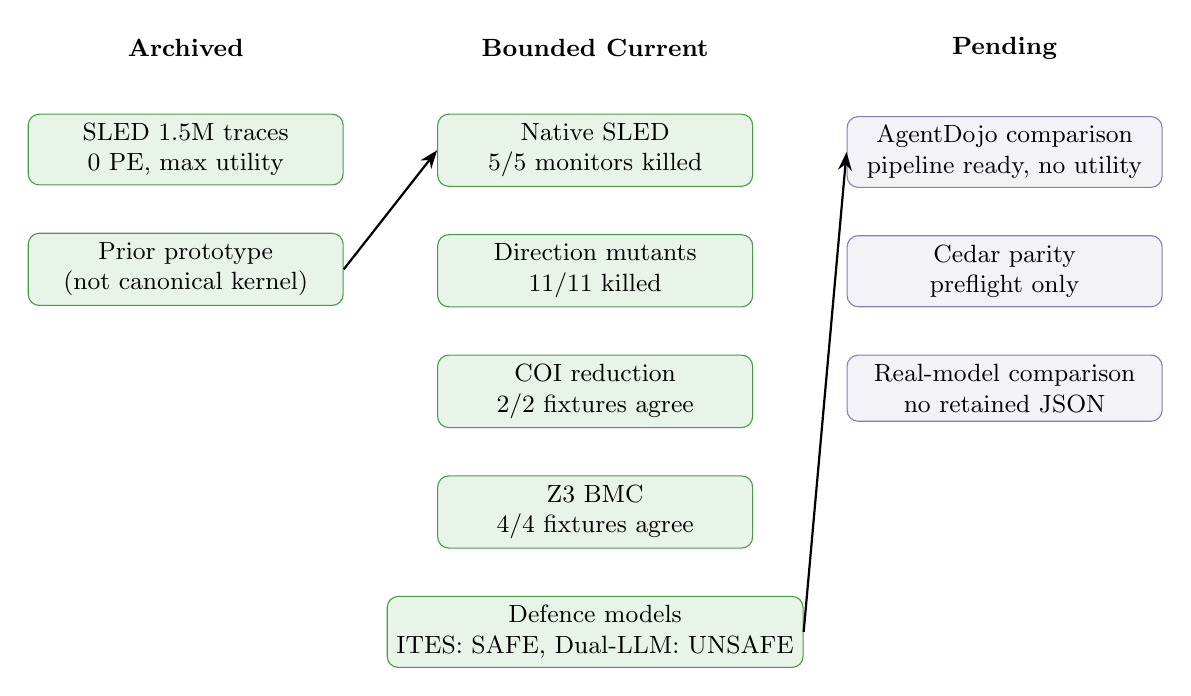
\begin{tikzpicture}[
  node distance=0.6cm and 1.2cm,
  tier/.style={draw, rounded corners, minimum width=4cm, minimum height=0.7cm,
              font=\small, align=center},
  safe/.style={fill=safebg!60, draw=safebd},
  unsafe/.style={fill=unsafebg!60, draw=unsafebd},
  pending/.style={fill=pendingbg!60, draw=pendingbd},
  label/.style={font=\small\bfseries, align=center},
]
\begin{scope}[]
% Colors are defined globally in the preamble

% Tier labels
\node[label] (al) at (0, 3.5) {Archived};
\node[label] (bl) at (5.2, 3.5) {Bounded Current};
\node[label] (cl) at (10.4, 3.5) {Pending};

% Archived column
\node[tier, safe, below=of al] (a1) {SLED 1.5M traces\\0 PE, max utility};
\node[tier, safe, below=of a1] (a2) {Prior prototype\\(not canonical kernel)};

% Bounded current column
\node[tier, safe, below=of bl] (b1) {Native SLED\\5/5 monitors killed};
\node[tier, safe, below=of b1] (b2) {Direction mutants\\11/11 killed};
\node[tier, safe, below=of b2] (b3) {COI reduction\\2/2 fixtures agree};
\node[tier, safe, below=of b3] (b4) {Z3 BMC\\4/4 fixtures agree};
\node[tier, safe, below=of b4] (b5) {Defence models\\ITES: SAFE, Dual-LLM: UNSAFE};

% Pending column
\node[tier, pending, below=of cl] (c1) {AgentDojo comparison\\pipeline ready, no utility};
\node[tier, pending, below=of c1] (c2) {Cedar parity\\preflight only};
\node[tier, pending, below=of c2] (c3) {Real-model comparison\\no retained JSON};

% Arrows between tiers
\draw[-Stealth, thick] (a2.east) -- (b1.west);
\draw[-Stealth, thick] (b5.east) -- (c1.west);
\end{scope}
\end{tikzpicture}
\caption{Evidence tiers: archived prototype results, bounded current
verification on finite models, and pending tracks gated on retained
result artefacts.  Green indicates SAFE or killed; grey indicates
evaluation-ready but no result.}
\label{fig:evidence-tiers}
\end{figure}


% GENERATED FILE -- do not edit by hand.
% Source: output\runs\native-sled-reproduction-v1\result.json; output\runs\direction-readiness-v1\security-mutations.json; output\runs\sled-coi-reduction-v1\result.json; output\runs\agentdojo-1b5-nf4-v1\result.json
% SHA-256: 0aa8c0a41bc8b6da960ecb52ed0dca2f21c99853aa768a4fca9dd8e00ca87e1a
% Run: python scripts/generate_paper_figures.py

\begin{table}[h]
\centering
\small
\begin{tabular}{p{3.5cm}p{2.5cm}p{3.5cm}p{3cm}}
\toprule
Evidence & Tier & Result & Limitation \\
\midrule
Archived SLED (1.5M traces) & Archived & 0 PE, maximal utility & Prior prototype, not canonical kernel \\
Repository validation & Current & 220 tests, 90.25\% branch coverage & Assumes complete mediation \\
Native SLED reproduction & Bounded & 5/5 monitors detected, 1-step witnesses & Finite fixtures only \\
Direction readiness & Bounded & 11 mutants killed, 1-step witnesses & Finite disclosure/delegation models \\
COI reduction & Bounded & 2 fixtures agree, Z3 confirms equivalence & Finite IR models \\
AgentDojo translation & Current & 6-cell pipeline runs end-to-end & 1.5B model too small for utility \\
Cedar differential & Pending & Preflight validates corpus; Cedar unavailable & No parity result \\
Real-model comparison & Pending & Pipeline ready & No retained result JSON \\\\
\bottomrule
\end{tabular}
\caption{Evidence status across archived, current, and pending results.
All numerical values are generated from versioned result JSON.}
\label{tab:evidence}
\end{table}


\subsection{Native SLED Reproduction}

The retained native reproduction detects all five seeded monitor defects,
each with a one-step witness, across three fixture pairs with fixed finite
bounds. This is bounded evidence: it exercises finite monitor models, not
all deployment observers.

\subsection{Direction Readiness}

The retained direction-readiness bundle reports safe exhaustion for the
canonical finite disclosure and delegation models and minimal witnesses for
every seeded selector, disclosure, attribution, and delegation defect.
Delegation remains disabled at runtime.

% GENERATED FILE -- do not edit by hand.
% Source: output\runs\direction-readiness-v1\security-mutations.json
% SHA-256: dbb42f6c9d0ac2d5e13482a365e58fecf874b8d6a2f5b45e70064271703c0fed
% Run: python scripts/generate_paper_figures.py

\begin{figure}[t]
\centering
\small
\begin{tabular}{lllcc}
\toprule
Category & Mutation & Property violated & Witness & Killed \\
\midrule
delegation & widened\_scope & delegation\_attenuated & 1 & \textcolor{red!70}{$\times$} \\
delegation & wrong\_beneficiary & delegation\_beneficiary\_bound & 1 & \textcolor{red!70}{$\times$} \\
delegation & reuse & delegation\_single\_use & 1 & \textcolor{red!70}{$\times$} \\
delegation & expiry\_bypass & delegation\_expiry\_enforced & 1 & \textcolor{red!70}{$\times$} \\
delegation & revocation\_bypass & delegation\_revocation\_enforced & 1 & \textcolor{red!70}{$\times$} \\
delegation & redelegation & delegation\_not\_redelegated & 1 & \textcolor{red!70}{$\times$} \\
delegation & post\_influence\_issuance & delegation\_precedes\_influence & 1 & \textcolor{red!70}{$\times$} \\
disclosure & unauthorised\_selector & no\_unauthorised\_selector & 1 & \textcolor{red!70}{$\times$} \\
disclosure & hidden\_error\_leak & no\_hidden\_decision\_leakage & 1 & \textcolor{red!70}{$\times$} \\
disclosure & incomplete\_attribution & complete\_attribution & 1 & \textcolor{red!70}{$\times$} \\
disclosure & unsafe\_redaction & no\_hidden\_decision\_leakage & 1 & \textcolor{red!70}{$\times$} \\
\bottomrule
\end{tabular}
\caption{Direction-readiness mutation testing: all 11 seeded defects
(7 delegation, 4 disclosure) are killed with one-step witnesses.
``$\times$'' denotes UNSAFE (counterexample found); all canonical
models exhaust SAFE.}
\label{fig:mutation-matrix}
\end{figure}


\subsection{AgentDojo Translation Boundary}

AgentDojo is pinned to package 0.1.35 and benchmark v1.2.2. The retained
fixture proves translation only; a live no-defence-versus-ITES comparison
is pending. A pilot run with Qwen2.5-1.5B-Instruct NF4 completed all six
protocol cells end-to-end, but the model is too small to complete tasks;
this is pipeline-readiness evidence, not a utility claim.

% GENERATED FILE -- do not edit by hand.
% Source: output\runs\agentdojo-1b5-nf4-v1\result.json
% SHA-256: 0f20267de2526bbb2931f3515ab0801a34d93251bbe3f91b34906d5c191b3d8d
% Run: python scripts/generate_paper_figures.py

\begin{figure}[t]
\centering
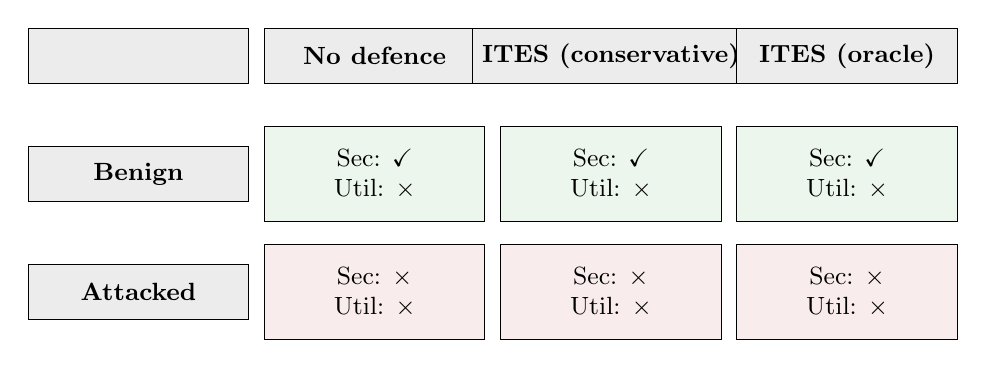
\begin{tikzpicture}[
  cell/.style={draw, minimum width=2.8cm, minimum height=1.2cm,
              font=\small, align=center},
  header/.style={draw, minimum width=2.8cm, minimum height=0.7cm,
                font=\small\bfseries, fill=gray!15, align=center},
  safe/.style={fill=safebg!50},
  unsafe/.style={fill=unsafebg!50},
]
% Colors defined globally in preamble

% Headers
\node[header] (h0) at (0, 0) {};
\node[header] (h1) at (3, 0) {No defence};
\node[header] (h2) at (6, 0) {ITES (conservative)};
\node[header] (h3) at (9, 0) {ITES (oracle)};

% Row labels
\node[header] (r0) at (0, -1.5) {Benign};
\node[header] (r1) at (0, -3) {Attacked};

% Cells - Benign
\node[cell, safe] at (3, -1.5) {Sec: \checkmark\\Util: $\times$};
\node[cell, safe] at (6, -1.5) {Sec: \checkmark\\Util: $\times$};
\node[cell, safe] at (9, -1.5) {Sec: \checkmark\\Util: $\times$};

% Cells - Attacked
\node[cell, unsafe] at (3, -3) {Sec: $\times$\\Util: $\times$};
\node[cell, unsafe] at (6, -3) {Sec: $\times$\\Util: $\times$};
\node[cell, unsafe] at (9, -3) {Sec: $\times$\\Util: $\times$};
\end{tikzpicture}
\caption{AgentDojo six-cell pipeline matrix (Qwen2.5-1.5B-Instruct NF4).
All cells completed end-to-end.  Under attack, security fails for all
three defence variants because the 1.5B model produces invalid output;
this is pipeline-readiness evidence, not a utility or efficacy claim.}
\label{fig:agentdojo}
\end{figure}



\section{Discussion and Limitations}

Conflux assumes sound authentication, provenance, policy state, and complete
mediation. It does not prevent actions authorised for every influencing
principal and does not guarantee subjective intent alignment. Conservative
contexts can over-approximate influence, reducing utility. The
authority-intersection rule is structurally analogous to Biba's
low-water-mark contamination \citep{biba1977} and is a standard meet in
the powerset lattice \citep{denning1976}; novelty claims must be qualified
against the classical IFC literature
\citep{sabelfeld2003,myersliskov,declassification-survey,robust-declassification,attacker-control,nonmalleable-ifc}.

Authorised-read safety is not noninterference: a system can obey local ACL
checks and still leak information through outputs or control flow. Formal
results are scoped to their finite model, backend, and conformance
evidence. Delegation has a bounded model and lifecycle representation but
remains unsupported by operational ITES. Provider adapters are research
prototypes, not production isolation boundaries. Real-model, AgentDojo, and
planning comparisons remain pending until gated runs produce retained
evidence.


\section{Conclusion}

We have presented a unified view of ITES and SLED---from the original
theoretical guarantees and prototype evaluation through the Conflux
canonical reimplementation with independent policy ports, argument-aware
authorisation, controlled disclosure, structured attribution, authenticated
dynamic planning, serialisable formal verification, and a disabled
scoped-delegation foundation. The core security guarantee---that authority
can only decrease as influence accumulates---follows from the
provenance-based authorisation rule and is independent of language-model
behaviour. The remaining research contribution is stronger evidence and
carefully gated activation: real-model, external-benchmark, and formal
artefacts whose claims remain tied to explicit assumptions, models, and
bounds.


\begin{ack}
Removed for double-blind review.
\end{ack}


\bibliography{references}
\bibliographystyle{plainnat}


\appendix
\input{checklist}


\end{document}
